{\em Square Killer} ist eine Variante von Sudoku, die auf einem
$n^2\times n^2$ Spielfeld gespielt wird.
Die normalen Sudoku-Regeln gelten, zusätzlich muss aber die Zahl
der Ziffern in einem zusammenhängenden grauen Gebiet (``Käfig'')
eine Quadratzahl sein.

Das besondere an dieser Variante ist, dass es Square~Killer-Rätsel gibt, die
ganz ohne Vorgabe-Zahlen auskommen, zum Beispiel:
\begin{center}
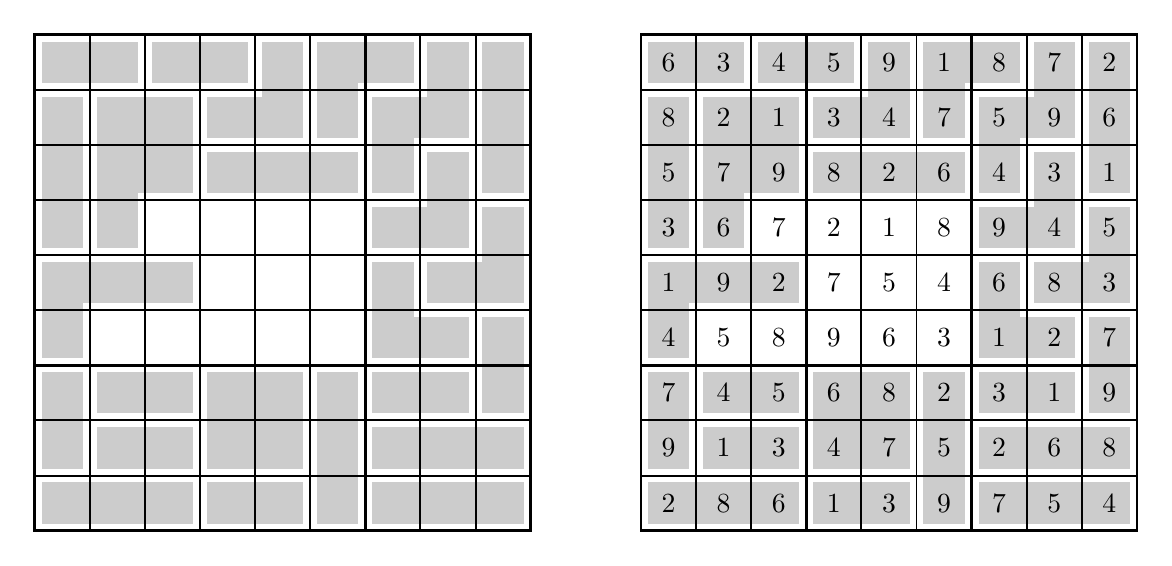
\begin{tikzpicture}[>=latex,thick,scale=0.7]

\def\squarekiller{
\fill[color=gray!40] (0,0) rectangle (9,9);

\fill[color=white] (3,3) rectangle (6,6);
\fill[color=white] (2,5) rectangle (3,6);
\fill[color=white] (1,3) rectangle (3,4);

\draw[color=white,line width=5pt] (0,8) rectangle (2,9);
\draw[color=white,line width=5pt] (2,8) rectangle (4,9);
\draw[color=white,line width=5pt] (3,7)--(5,7)--(5,9)--(4,9)--(4,8)--(3,8)--cycle;
\draw[color=white,line width=5pt] (5,7)--(6,7)--(6,8)--(7,8)--(7,9)--(5,9)--cycle;
\draw[color=white,line width=5pt] (6,6)--(7,6)--(7,7)--(8,7)--(8,9)--(7,9)--(7,8)--(6,8)--cycle;
\draw[color=white,line width=5pt] (8,6) rectangle (9,9);
\draw[color=white,line width=5pt] (3,6) rectangle (6,7);
\draw[color=white,line width=5pt] (0,5) rectangle (1,8);
\draw[color=white,line width=5pt] (1,5)--(2,5)--(2,6)--(3,6)--(3,8)--(1,8)--cycle;
\draw[color=white,line width=5pt] (6,5)--(8,5)--(8,7)--(7,7)--(7,6)--(6,6)--cycle;
\draw[color=white,line width=5pt] (7,4)--(9,4)--(9,6)--(8,6)--(8,5)--(7,5)--cycle;
\draw[color=white,line width=5pt] (0,3)--(1,3)--(1,4)--(3,4)--(3,5)--(0,5)--cycle;
\draw[color=white,line width=5pt] (6,3)--(8,3)--(8,4)--(7,4)--(7,5)--(6,5)--cycle;
\draw[color=white,line width=5pt] (1,2) rectangle (3,3);
\draw[color=white,line width=5pt] (6,2) rectangle (8,3);
\draw[color=white,line width=5pt] (8,2) rectangle (9,4);
\draw[color=white,line width=5pt] (0,1) rectangle (1,3);
\draw[color=white,line width=5pt] (1,1) rectangle (3,2);
\draw[color=white,line width=5pt] (3,1) rectangle (5,3);
\draw[color=white,line width=5pt] (6,1) rectangle (9,2);
\draw[color=white,line width=5pt] (0,0) rectangle (3,1);
\draw[color=white,line width=5pt] (3,0) rectangle (5,1);
\draw[color=white,line width=5pt] (5,0) rectangle (6,3);
\draw[color=white,line width=5pt] (6,0) rectangle (9,1);

\draw[line width=1pt] (0,0) rectangle (9,9);
\foreach \x in {1,...,8} {
	\draw[line width=0.7pt] (\x,0) -- (\x,9);
	\draw[line width=0.7pt] (0,\x) -- (9,\x);
}
\foreach \x in {3,6}{
	\draw[line width=1.0pt] (\x,0) -- (\x,9);
	\draw[line width=1.0pt] (0,\x) -- (9,\x);
}
}

\begin{scope}[xshift=-5.5cm]
\squarekiller
\end{scope}

\begin{scope}[xshift=5.5cm]
\squarekiller
\def\feld#1#2#3{
	\node at ({#1-0.5},{#2-0.5}) {$#3$};
}

\feld{1}{1}{2}
\feld{2}{1}{8}
\feld{3}{1}{6}
\feld{4}{1}{1}
\feld{5}{1}{3}
\feld{6}{1}{9}
\feld{7}{1}{7}
\feld{8}{1}{5}
\feld{9}{1}{4}

\feld{1}{2}{9}
\feld{2}{2}{1}
\feld{3}{2}{3}
\feld{4}{2}{4}
\feld{5}{2}{7}
\feld{6}{2}{5}
\feld{7}{2}{2}
\feld{8}{2}{6}
\feld{9}{2}{8}

\feld{1}{3}{7}
\feld{2}{3}{4}
\feld{3}{3}{5}
\feld{4}{3}{6}
\feld{5}{3}{8}
\feld{6}{3}{2}
\feld{7}{3}{3}
\feld{8}{3}{1}
\feld{9}{3}{9}

\feld{1}{4}{4}
\feld{2}{4}{5}
\feld{3}{4}{8}
\feld{4}{4}{9}
\feld{5}{4}{6}
\feld{6}{4}{3}
\feld{7}{4}{1}
\feld{8}{4}{2}
\feld{9}{4}{7}

\feld{1}{5}{1}
\feld{2}{5}{9}
\feld{3}{5}{2}
\feld{4}{5}{7}
\feld{5}{5}{5}
\feld{6}{5}{4}
\feld{7}{5}{6}
\feld{8}{5}{8}
\feld{9}{5}{3}

\feld{1}{6}{3}
\feld{2}{6}{6}
\feld{3}{6}{7}
\feld{4}{6}{2}
\feld{5}{6}{1}
\feld{6}{6}{8}
\feld{7}{6}{9}
\feld{8}{6}{4}
\feld{9}{6}{5}

\feld{1}{7}{5}
\feld{2}{7}{7}
\feld{3}{7}{9}
\feld{4}{7}{8}
\feld{5}{7}{2}
\feld{6}{7}{6}
\feld{7}{7}{4}
\feld{8}{7}{3}
\feld{9}{7}{1}

\feld{1}{8}{8}
\feld{2}{8}{2}
\feld{3}{8}{1}
\feld{4}{8}{3}
\feld{5}{8}{4}
\feld{6}{8}{7}
\feld{7}{8}{5}
\feld{8}{8}{9}
\feld{9}{8}{6}

\feld{1}{9}{6}
\feld{2}{9}{3}
\feld{3}{9}{4}
\feld{4}{9}{5}
\feld{5}{9}{9}
\feld{6}{9}{1}
\feld{7}{9}{8}
\feld{8}{9}{7}
\feld{9}{9}{2}

\end{scope}


\end{tikzpicture}
\end{center}

Kann eine nichtdeterministische Turing-Maschine in polynomieller
Zeit entscheiden, ob ein {\em Square Killer}-Rätsel eine Lösung hat?

\thema{NP}
\thema{polynomieller Verifizierer}

\begin{loesung}
Das Problem ist natürlich entscheidbar, man kann die endlich vielen
möglichen Zahlenverteilungen durchprobieren und die Regeln überprüfen.

Die Fragestellung ist gleichbedeutend mit der Frage, ob es einen
polynomiellen Verifizierer gibt.

Für einen polynomiellen Verifizierer brauchen wir ein Lösungszertifikat,
wir nehmen dafür die Zahlen, die in den Feldern stehen.
Folgende Verifikationsschritte sind noch nötig:
\begin{center}
\begin{tabular}{c|p{8cm}|r}
Nummer&Verifikation&Zeit\\
\hline
1&Sudoku-Verifizierer&polynomiell\\
2&Für jedes Feld überprüfen, ob die Summe der Zahlen im gleichen Käfig
eine Quadratzahl ist.
&$O(n^4)\cdot O(n^4)$\\
\hline
&Total&polynomiell
\end{tabular}
\end{center}
Die Laufzeit dieses Verifizierers ist polynomiell.
\end{loesung}

\begin{diskussion}
Das vorgestellte Beispiel stammt von Christoph Seeliger und wird von
{\em Cracking the Cryptic} im Video
\url{https://www.youtube.com/watch?v=myGqOF6blPI}
live gelöst.
\end{diskussion}

\begin{bewertung}
Entscheidbarkeit ({\bf E}) 1 Punkt,
Verifizierer ({\bf V}) 1 Punkt,
Zertifikat ({\bf Z}) 1 Punkt,
bestehende Sudoku Regeln sind in polynomieller Zeit verifizierbar
({\bf S}) 1 Punkt,
Verifikation von zwei zusätzlichen Regel ({\bf R}) 1 Punkt,
Laufzeit polynomiell ({\bf L}) 1 Punkt.
\end{bewertung}

